\chapter{Versuche mit dem MEMS-Sensor} 
	In einem weiteren Schritt soll ein MEMS-Sensor in Betrieb genommen werden, welcher im Produkt angewendet wird. 
	\section{Versuchsaufbau}
	Die Versuche mit den piezoelektrischen Sensoren \ref{subsec:signale} haben gezeigt, dass
	Beschleunigungen �ber 100g gemessen werden. Deshalb wurde besonders auf einen grossen
	Dynamikbereich geachtet. Ausserdem muss die Abtastfrequenz �ber 100Hz liegen. Es wurde der Sensor
	H3LIS331DL von STMicroelectronics eingesetzt. Dieser hat einen einstellbaren Bereich von $\pm100g$,
	$\pm200g$ und $\pm400g$. Die Daten werden digitalisiert. Es kann �ber I2C oder SPI mit dem Sensor
	kommuniziert werden. Die Abtastfrequenz kann zwischen 0.5Hz bis 1kHz konfiguriert werden. Der
	Sensor ist mit der Gr�sse von 3x3x1mm$^2$ sehr klein. Zwei Interruptausg�nge k�nnen konfiguriert
	werden. Eine M�glichkeit ist beispielsweise, dass ein �berschreiten eines Schwellwerts angezeigt
	wird. Weitere Eigenschaften des Sensors k�nnen dem Datenblatt \cite{H3L} entnommen werden.
	
	Als zweite Komponente wurde ein FRDM-K64F Freedom Board verwendet. Dieses bietet neben der 
	Konfiguration des Sensors die M�glichkeit, die ausgelesenen Daten auf einer SD-Karte zu speichern. 
	
	Mit einer Power Bank kann das Freedom Board und der Sensor gespeist werden. So bleibt die Messeinheit
	mobil. 
	\begin{figure}
		\centering
		%\vspace{-1cm}
		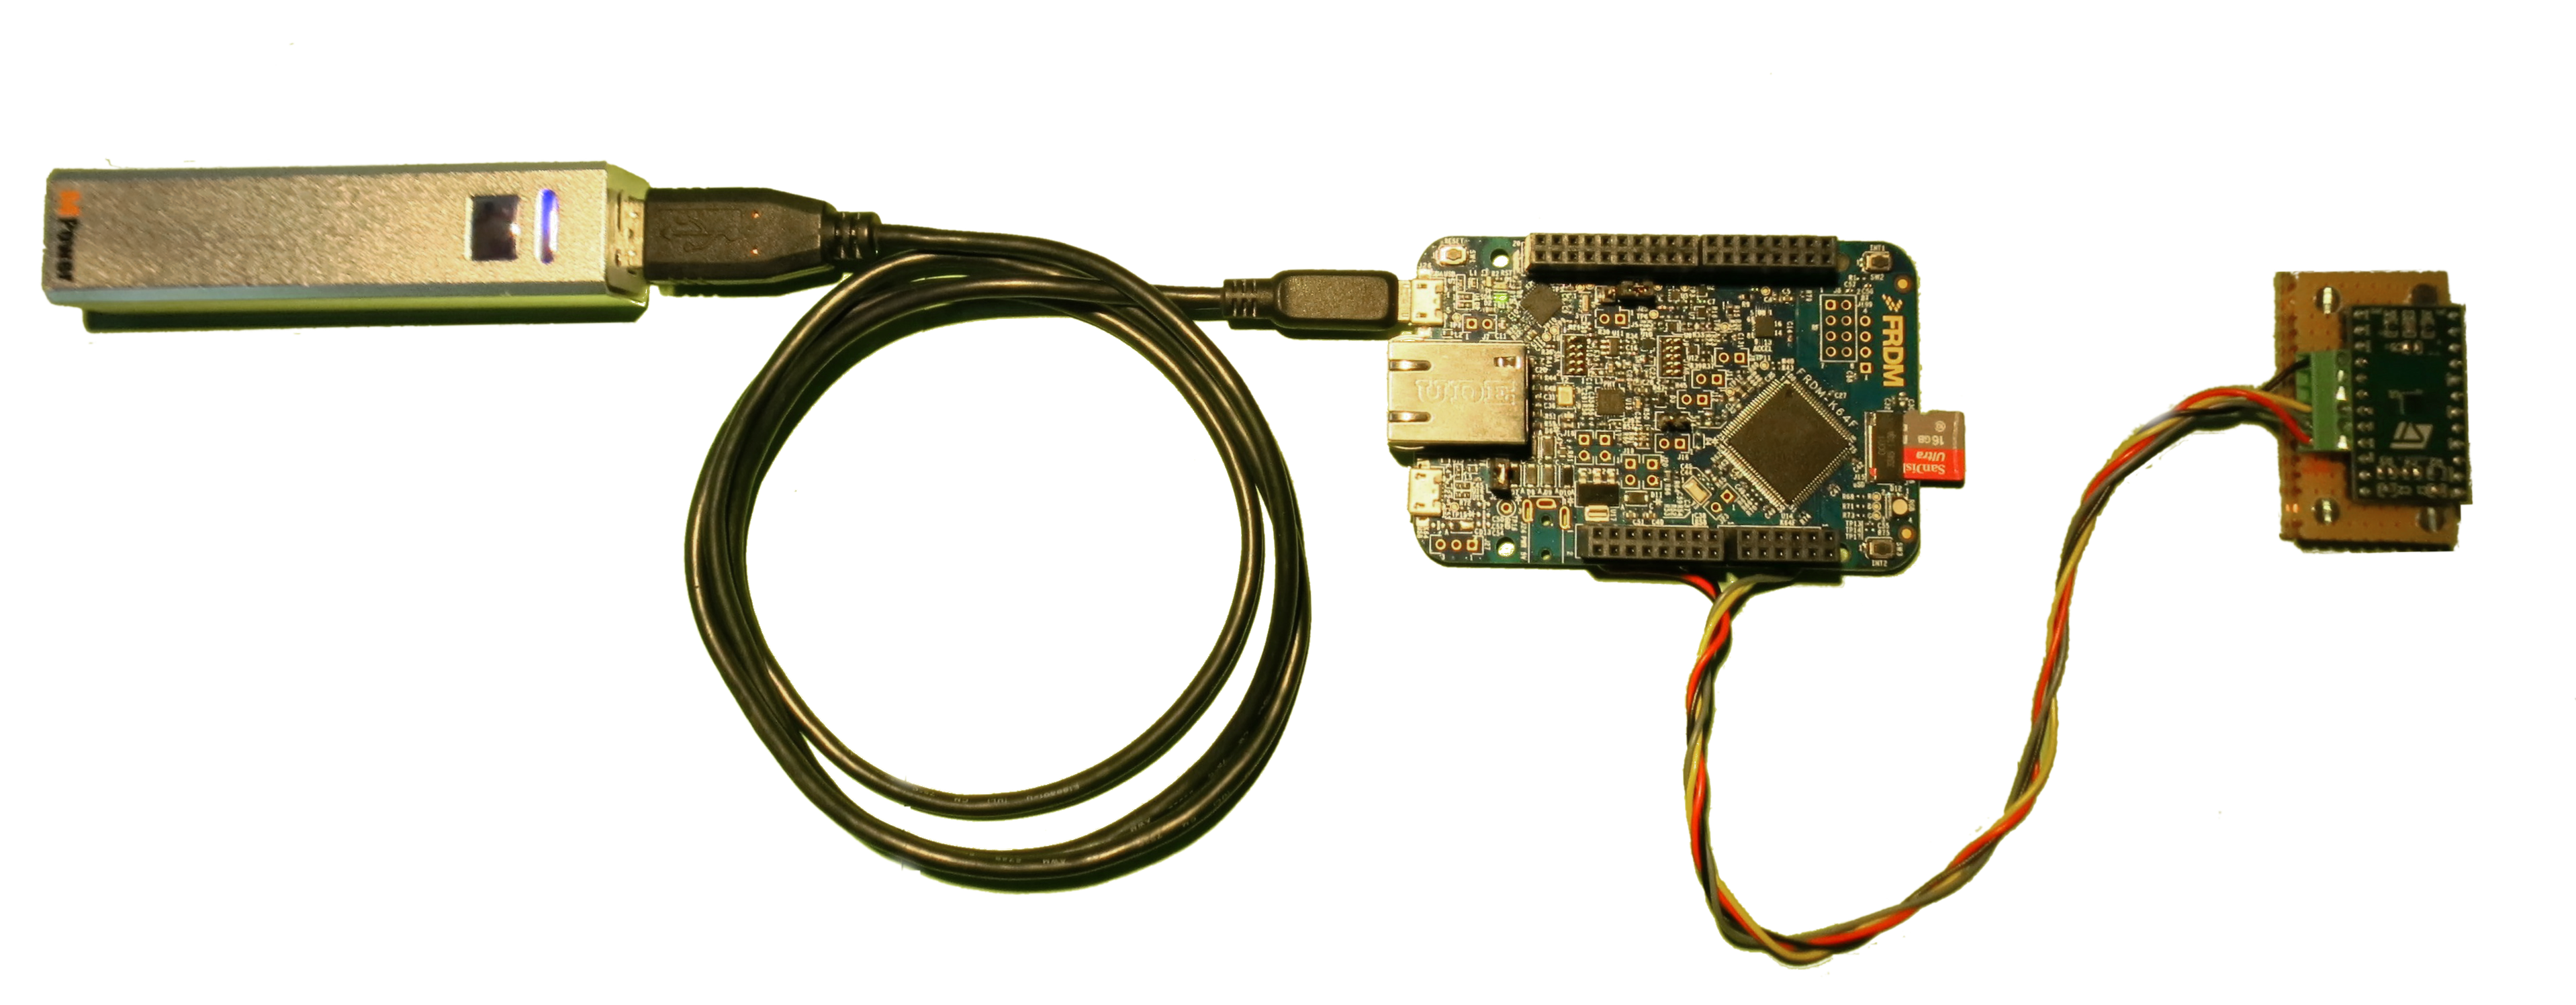
\includegraphics[width=15cm]{img/mems_aufbau.png}
		\caption{Der Aufbau mit MEMS-Sensor, Freedom Board und Power Bank}
		\label{fig:mems_aufbau}
	\end{figure}
	
	\subsection{Aufbau der Software}
	F�r die Software wurde FreeRTOS verwendet. Die Software ist in drei Tasks aufgebaut. Der Idle-Task
	wird immer dann ausgef�hrt, wenn kein anderer Task die CPU ben�tigt. Der Main-Task hat die Aufgabe,
	die Tasten zu pollen und die Events zu handeln. Wichtiger f�r den Aufbau der Software ist der
	Sensor-Task und der SD-Karten-Task. Der Sensor-Task kommuniziert �ber I2C mit dem Sensor und liest
	Daten, falls vorhanden, vom Sensor aus. Er speichert ausserdem diese Daten in einer Queue. Der
	SD-Karten-Task wiederum liest die Daten aus der \index{Queue}, speichert diese in einem Buffer als String.
	Ist der Buffer voll, wird dieser auf die SD-Karte gespeichert.
	
	Im Sensor-Task und im SD-Karten-Task werden Zustandsautomaten durchgearbeitet. Diese k�nnen einerseits
	durch Tastendr�cke oder Interne Signale beeinflusst werden. Die Kommunikation zwischen dem Main-Task,
	dem Sensor-Task und dem SD-Karten-Task erfolgt dabei mittels Task Notifications. 
	
	Task Notifications gibt es ab FreeRTOS-Version V8.2.0 (16. Januar 2015). Sie dienen dienen der
	Inter-Task-Kommunikation und Synchronisation, �hnlich den Semaphoren. Jeder Task hat dabei einen
	32-bit notification value. In dieser Anwendung wurde jeweils ein Bit des notification values einem
	Tastendruck oder einem internen Signal zugewiesen. Der Main-Task setzt beispielsweise bei einem
	Tastendruck des Button 2 das erste Bit im notification value. Der Sensor-Task wechselt seinen
	Zustand von "'IDLE"' in "'MEASURE"', wenn dieses Bit gesetzt wurde. Task Notifications sind
	effizienter als Semaphoren \cite{TaskNotification}. 

	Die \autoref{fig:sm_sensor} und \autoref{fig:sm_sd} veranschaulichen die beiden Zustandsautomaten. 
	\begin{figure}
		\centering
		%\vspace{-1cm}
		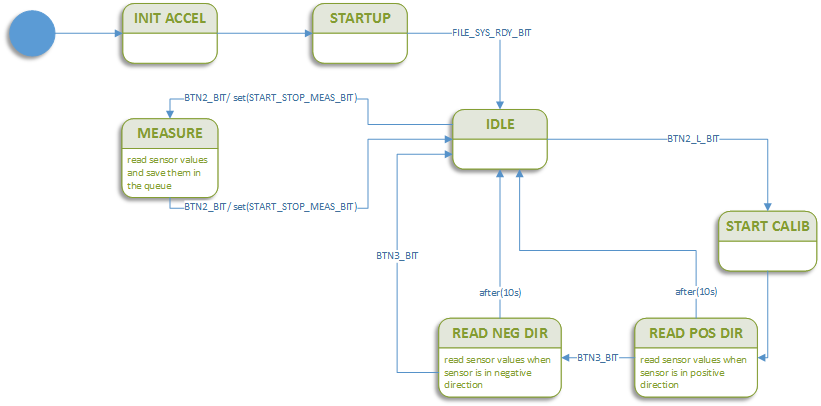
\includegraphics[width=15cm]{img/sm_sensor.png}
		\caption{Zustandsdiagramm Sensor-Task}
		\label{fig:sm_sensor}
	\end{figure}
	
	Der Zustandsautomat durchl�uft den Zustand "'INIT ACCEL"' in welchem der Sensor konfiguriert 
	wird. Zuerst wird getestet, ob der Sensor antwortet. Dann werden der Messbereich, die Abtastrate, 
	der Power-Modus und die Art der Datenaufbereitung eingestellt. Der Sensor kann im Normal Powermodus
	betrieben werden, oder aber in verschiedenen Low Powermoden. In den Low Powermoden ist die 
	Abtastrate nicht konfigurierbar und tiefer als im Normal Powermodus. Die Beschleunigungsdaten des Sensors werden 
	in zwei 8-bit Registern abgelegt. 
	
	Nachdem der Sensor konfiguriert ist, wechselt der Zustandsautomat in den Zustand "STARTUP". Hier wird
	so lange gewartet, bis der SD-Karten-Task mit einer Task Notification bekannt gibt, dass er das File 
	System gemounted hat. 
	
	Der Zustandsautomat im Sensor-Task hat grunds�tzlich zwei Schlaufen. Zum einen kann durch einen 
	Tastendruck des Buttons 2 die Messung gestartet w
	\begin{figure}
		\centering
		%\vspace{-1cm}
		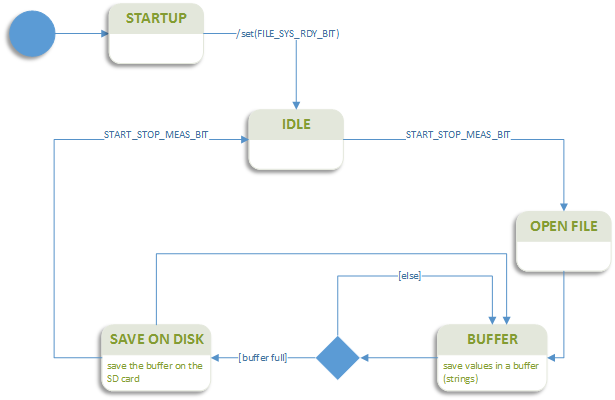
\includegraphics[width=12cm]{img/sm_sd.png}
		\caption{Zustandsdiagramm SD-Karten-Task}
		\label{fig:sm_sd}
	\end{figure}